\chapter{ Simplicial complex as Higher-order Topology Description } \label{chap:SC}

\lhead{\emph{Simplicial complexes}}



\section{ From graph to higher-order models } \label[section]{sec:higher-order-models}

\todo{graph definition}

\todo{graph examples in real life (2 or 3)}

\todo{motivation for the transition to the higher order models}

\todo{Hypergraphs: definitions and examples}

\todo{Motifs: definitions and examples}

\todo{somehow relate to the tensor models and tractability
simplicial complexes}












\section{ Simplicial Complexes } \label[section]{sec:SCs}


Let \( V = \{ v_1, v_2, \ldots, v_n \} \) be a set of nodes; as discussed above, such set may refer to various interacting entities and agents in the system, e.g.\ neurons, genes, traffic stops, online actors, publication authors, etc. Then: 

\begin{definition}[Simplicial Complex]\label[definition]{def:simplicial_complex}
      The collection of subsets \( \mathcal K \) of the nodal set \( V \) is  a (abstract) {SC}\footnote{addition of the word ``abstract'' to the term is more common in the topological setting} if for each subset \( \sigma \in \mc K \), referred as a {simplex}, all its subsets \( \sigma'\), \( \sigma' \subseteq \sigma \), referred as {faces}, enter \( \mc K \) as well, \( \sigma' \in \mc K\).
\end{definition}

We denote simplex \( \sigma \) on the set of vertices \( \{ u_1, u_2, \dots u_{k+1} \} \in V  \) as \( \sigma = [u_1, u_2, \dots u_{k+1} ]\). Then, a simplex \( \sigma \in \mc K \) on \( k + 1 \) vertices is said to be of the order \( k \), \( \ord \sigma = k \); alternatively, we refer to it as a \(k\)-order simplex or \(k\)-simplex. Let \( \V k \) be a set of all \(k\)-order simplices in \( \mc K \) and \( m_k \) is the cardinality of \( \V k\), \( m_k = | \V k | \); then \( \V 0 \) is the set of nodes in the simplicial complex \( \mc K \), \( \V 1 \) --- the set of edges, \( \V 2 \) --- the set of triangles, or \(3\)-cliques, and so on, with \( \mc K = \{ \V 0, \V 1, \V 2 \ldots \} \). Note that due to the inclusion rule in \Cref{def:simplicial_complex}, the number of non-empty \( \V k \) is finite and, moreover, uninterupted in a sense of the order: if \( \V k = \vn \), then \( \V {k+1} \) is also necessarily empty.
\begin{definition}[\(k\)-skeleton]\label[definition]{def:skeleton}
      For a given simplicial complex \( \mc K \), a \(k\)-skeleton is defined as a simplicial complex \( \mc K^{(k)} \) containing all simplices of \( \mc K \) of order at most \( k \), 
      \begin{equation}
            \mc K^{(k)} = \cup_{i=0}^k \V i
      \end{equation}
      For instance, \( 2 \)-skeleton of \( \mc K \) consists of all nodes, edges and triangles of \( K \).
\end{definition}

It is easy to note that \( k\)-skeleton remains a simplicial complex: if \( \sigma \in K^{(k)}\), then all simplices \( \tau \) from the original complex \( \mc K \), \( \ord \tau \le \ord \sigma \), belong to \( \mc K^{(k)} \) by definition; then, by inclusion principle, all faces \( \sigma' \) of \( \sigma \) belong to \( \mc K \) and \( \ord \sigma' < \ord \sigma \le k \), so all faces of \( \sigma \) are necessarily included in the \( k\)-skeleton.

\begin{figure}[hbtp]
      \centering
      \begin{tikzpicture}

      \fill [opacity=0.3,liberty]    (0, 0) -- (3, 0) --  (1.5, 2.6) -- cycle;
      %\node at (1.5, 0.9) {\AxisRotator[rotate=-90]};
      %\node at (1.5, 1.2) {\small \color{liberty!50!jet} +1};
      \fill [opacity=0.2,liberty]    (5.0, 1.0) -- (6.5, 2.6) --  (6.4, 1.4) -- cycle;
      %\node at (17.9/3, 5/3) {\AxisRotatorMirror[rotate=0]};
      \fill [opacity=0.6,liberty]    (5.0, 1.0) -- (9.0, -0.4) --  (6.4, 1.4) -- cycle;
      %\node at (6.8, 2/3) {\AxisRotator[rotate=-90]};
      \fill [opacity=0.4,liberty]    (6.5, 2.6) -- (9.0, -0.4) --  (6.4, 1.4) -- cycle;
      %\node at (7.3, 1.2) {\AxisRotatorMirror[rotate=-90]};
      
      


      \Vertex[x=0, y=0,style={color=persimmon}, fontcolor=white, size=0.25, label = 1]{v1}
      %\node[below left=-1pt of v1] {\small \color{persimmon}+1};
      \Vertex[x=3, y=0,style={color=persimmon}, fontcolor=white, size=0.25, label = 2]{v2}
      %\node[below=-1pt of v2] {\small \color{persimmon}-2};
      \Vertex[x=1.5, y=2.6, style={color=persimmon}, fontcolor=white, size=0.25, label = 3]{v3}
     % \node[above=-1pt of v3] {\small \color{persimmon}+0};
      \Vertex[x=5, y=1.0, style={color=persimmon}, fontcolor=white, size=0.25, label = 4]{v4}
    %  \node[above=-1pt of v4] {\small \color{persimmon}-3};
      \Vertex[x=6.5, y=2.6, style={color=persimmon}, fontcolor=white, size=0.25, label = 5]{v5}
   %   \node[above right=-1pt of v5] {\small \color{persimmon}-1};
      \Vertex[x=9, y=-.4, style={color=persimmon}, fontcolor=white, size=0.25, label = 6]{v6}
  %    \node[below=-1pt of v6] {\small \color{persimmon}+0};
      \Vertex[x=6.4, y=1.4, style={color=persimmon}, fontcolor=white, size=0.25, label = 7]{v7}
 %     \node[right=-1pt of v7] {\small \color{persimmon}+2};
      \Vertex[x=11.0, y=2.0, style={color=persimmon}, fontcolor=white, size=0.25, label = 8]{v8}
%      \node[above=-1pt of v8] {\small \color{persimmon}+3};

      \Edge[](v1)(v2)
      \Edge[](v1)(v3)
      \Edge[](v2)(v3)
      \Edge[](v2)(v4)
      \Edge[](v3)(v4)
      \Edge[](v4)(v5)
      \Edge[](v4)(v6)
      \Edge[](v4)(v7)
      \Edge[](v5)(v6)
      \Edge[](v5)(v7)
      \Edge[](v6)(v7)
      \Edge[](v6)(v8)
\end{tikzpicture}
      \caption{
            Example of a simplicial complex on \(8\) nodes; nodes included in the compelx are shown in orange, edges --- in black, and triangles  --- in blue.\label{fig:example_SC}}
\end{figure}


\begin{example}[Simplicial Complex]

      Here we provide the following example of the simplicial complex \( \mc K \), \Cref{fig:example_SC}: we denote \(0\)-order simplices (vertices) by orange color, \( 1\)-order simplicies (edges) by black and \( 2\)-order simplices (triangles) by blue, where: 
      \begin{equation}
            \begin{aligned}
                  \V 0 & = \{ [1], [2], [3], [4], [5], [6], [7], [8] \} \\
                  \V 1 & = \{ [1, 2], [1, 3], [2, 3], [2, 4], [3, 4], [4, 5], [4, 6], [4, 7], [5, 6], [5, 7], [6, 7], [6, 8] \} \\
                  \V 2 & = \{ [ 1, 2, 3 ], [4, 5, 7], [4, 6, 7], [5, 6, 7] \}
            \end{aligned}
      \end{equation}
      Note that \( \V 3 = \vn \), so the highest order of simplices in \( \mc K \) is \( 2 \). Additionally, edge \( [4, 5] \), \( [4, 6]\) and \( [5, 6]\) are included in \( \mc K \), but the triangle \( [4, 5, 6]\) is not; this does not violate the inclusion rule. Instead, every edge and every vertices of every triangle in \( \V 2 \) as well as every vertex of every edge in \( \V 1 \) are contained in \( \mc K \) fullfilling the inclusion principle.
\end{example}

\begin{example}[Real Life Simplicial Complex]

      coauthorship graph? cannot find a nice picture

      \todo{find a natural example of the simplicial complex with an illustration}
      
\end{example}


Comparing to the definition of the hypergraph above, it is easy to see that simplicial complex is a special case of a hypergraph where every edge is enclosed with respect to the inclusion (every subset of every hyperedge is a hyperedge). In other words, simplicial complex contains additional structural rigidness which allows to formally describe the topology of \( \mc K \); as a result, one is specifically interested in the formal desctiption of the nested inclusion principle achieved through \emph{boundary operators} defined in the subsections below.


Prior to discussing boundary mappings, we briefly cover the algebraic structure of such operators known as \emph{Hodge's theory}.

\section{ Hodge's Theory }

Two linear operators \( A \) and \( B \) are said to satisfy Hodge's theory if and only if their composition is a null operator, 
\begin{equation}
      A B = 0
\end{equation}
which is equivalent to \( \im B \subseteq \ker A \).

\begin{definition}\label[definition]{def:quotient}
      For a pair of operators \( A \) and \( B \) satisfying Hodge's theory, the \emph{quotient space} \( \mc H \) is defined as follows:
      \begin{equation}
            \mc H = \faktor{ \ker A }{\im B}
      \end{equation}
      where each element of \( \mc H \) is a manifold \( \b x + \im B = \left\{ \b x + \b y \mid \forall \b y \in \im B \right\}\) for \( \b x \in \ker A \). It follows directly from the definition that \( \mc H\) is an abelian group under addition.
\end{definition}

By \Cref{def:quotient}, the quotient space \( \mc H \) is a collection\todo{in a general sense} of \emph{equivalence classes} \( \b x + \im B \). Then, each class \( \b x + \im B = \b x_H + \im B \) for some \( \b x_H \perp \im B \) (both \( \b x, \b x_H \in \ker A \)); indeed, since the orthogonal component \( \b x_H \) (referred as \emph{harmonic representative}) of \( \b x \) with respect to \( \im B\) is unique, the map \( \b x_H \leftrightarrow \b x + \im B \) is bijectional.

\begin{figure}[hbtp]
      \centering
            \newcommand*{\xMin}{-1}%
\newcommand*{\xMax}{2}%
\newcommand*{\yMin}{-2}%
\newcommand*{\yMax}{2}%

\begin{tikzpicture}
      \foreach \i in {\xMin,...,\xMax} {
        \draw [very thin,lightgray] (\i,\yMin-0.2) -- (\i,\yMax+0.2)  node [below] at (\i,\yMin) {};
    }
    \foreach \i in {\yMin,...,\yMax} {
        \draw [very thin,lightgray] (\xMin-0.2,\i) -- (\xMax+0.2,\i) node [left] at (\xMin,\i) {};
    }

    \draw [gray] (\xMin-0.2, 0) -- (\xMax+0.2,0) node [left] at (\xMin,0) {};
    \draw [gray] (0,\yMin-0.2) -- (0,\yMax+0.2)  node [below] at (0,\yMin) {};
    \node at (-1.75, 1.75) { \large \(\ker A \)};

    \draw [black, line width = 3, dashed] (-1, -2) -- (1, 2) node [below] at (0.0, 1.75){ \large \( \im B \) };

    \draw [black, line width = 3] (0.25, -2) -- (2.25, 2) node [below] at (0.0, 1.75){ \large \( \im B \) };

    \draw [liberty, -{latex}, line width = 2] (0, 0) -- (1.15, 0) node [above] at (0.6, 0) {\large \( \b x \)};
    \draw [persimmon, -{latex}, line width = 2] (0, 0) -- (0.9, -.6) node [below] at (0.3, -0.3) {\large \( \b x_H \)};
\end{tikzpicture}
            \caption{Illustration of a harmonic representative for an equivalence class}
\end{figure}

\begin{theorem}[{\cite[Thm 5.3]{limHodgeLaplaciansGraphs2020}}]\label[theorem]{thm:two_kernels}
      Let \( A \) and \( B \) be linear operators, \( A B = 0 \). Then the homology group \( \mc H \) satisfies:
      \begin{equation}
            \mc H = \faktor{\ker A }{\im B } \cong \ker A \cap \ker B^\top,
      \end{equation}
      where \( \cong \) denotes the isomorphism.
\end{theorem}

\begin{proof}
      One builds the isomorphism through the harmonic representative, as discussed above. It sufficient to note that \( \b x_H \perp \im B \Leftrightarrow \b x_H \in \ker B^\top \) in order to complete the proof.
\end{proof}

\begin{lemma}[{\cite[Thm 5.2]{limHodgeLaplaciansGraphs2020}}]\label[lemma]{lemma:hodge_kernels}
      Let \( A \) and \( B \) be linear operators, \( A B = 0 \). Then:
      \begin{equation}
            \ker A \cap \ker B^\top = \ker \left( A^\top A + B B^\top \right)
      \end{equation}
      \vspace{-\baselineskip}
\end{lemma}

\begin{proof}
      Note that if \( \b x \in \ker A \cap \ker B^\top \), then \( \b x \in \ker A \) and \( \b x \ker B^\top \), so \( \b x \in \ker \left( A^\top A + B B^\top  \right)\). As a result, \( \ker A \cap \ker B^\top \subset \ker \left( A^\top A + B B^\top  \right)\).

      On the other hand, let \( \b x \in \ker \left( A^\top A + B B^\top \right)\), then
      \begin{equation}
            A^\top A \b x  + B B^\top \b x = 0
      \end{equation}
      Exploiting \( A B = 0 \) and multiplying the equation above by \( B^\top \) and \( A \) one gets the following:
      \begin{equation}
            \begin{aligned}
                  & B^\top B B^\top \b x = 0 \\
                  & A A^\top A \b x = 0 
            \end{aligned}
      \end{equation}
      Note that \( A A^\top A \b x = 0 \Leftrightarrow A^\top A \b x \in \ker A \), but \( A^\top A \b x \in \im A^\top \), so by Fredholm alternative, \( A^\top A \b x = 0\). Finally, for \( A^\top A \b x = 0\):
      \begin{equation}
             A^\top A \b x = 0  \Longrightarrow  \b x^\top A^\top A \b x = 0 \iff \| A \b x \|^2 = 0 \Longrightarrow \b x \in \ker A  
      \end{equation}
      Similarly, for the second equation, \( \b x \in \ker B^\top \) which completes the proof.
\end{proof}

\todo{
      Here we need some words about the transitions.
}


Since \( A B = 0\), \( B^\top A^\top = 0 \) or \( \im A^\top \subset \ker B^\top \). Then, exploiting \( \ds R^n = \ker A \oplus \im A^\top \): 
\begin{equation}
      \begin{aligned}
            \ker B^\top & = \ker B^\top \cap \ds R^n = \ker B^\top \cap \left( \ker A \oplus \im A^\top \right) = \\
            & = \left( \ker A \cap \ker B^\top \right) \oplus \left( \im A^\top \cap \ker B^\top \right)
      \end{aligned}
\end{equation}
Given \Cref{lemma:hodge_kernels}, \( \ker A \cap \ker B^\top = \ker \left(  A^\top A + B B^\top \right) \) and, since \( \im A^\top \subset \ker B^\top \), \( \im A^\top \cap \ker B^\top = \im A^\top \), yeilding the decomposition of  the whole space:
\begin{theorem}[Hodge Decomposition]\label[theorem]{thm:hodge_decomposition}
      Let \( A \) and \( B \) be linear operators, \( A B = 0 \). Then:
      \begin{equation}
            \ds R^n = \lefteqn{\overbrace{\phantom{\im A^\top \oplus  \ker \left( A^\top A + B B^\top \right)}}^{\ker B^\top}} \im A^\top \oplus
            \underbrace{\ker \left( A^\top A + B B^\top \right) \oplus  \im B}_{\ker A}
      \end{equation}
      \vspace{-\baselineskip}
\end{theorem}



%=================================================%
%                                                 %
%=================================================%


\section{ Boundary and Laplacian Operators }

\subsection{Boundary operators \( B_k \)}

Each simplicial complex \( \mc K \) has a nested structure of simplicies: indeed, if \( \sigma \) is a simplex of order \( k \), \( \sigma \in \V k \), then all of \( (k-1)\)-th order faces forming the boundary of \( \sigma \) also belong to \( \mc K \): for instance, for the triangle \( \{ 1, 2, 3  \} \) all the border edges \( \{ 1, 2\} \), \( \{ 1, 3\}\) and \( \{ 2, 3 \}\) are also in the simplicial complex, \Cref{fig:example_SC}. 

This nested property implies that one can build a formal map from a simplex to its boundary enclosed inside the simplicial complex. 

\begin{definition}[Chain spaces]
      Let \( \mc K \) be a simplicial complex; then the space \( \mc C_k \) of formal sums of simplices from \( \V k \) over real numbers is called \emph{a \( k\)-th chain space}.

\end{definition}


Chain spaces on its own are naturally present in the majority of the network models: \( \mc C_0 \) is a space of states of vertices (e.g. in the dynamical system \( \dot{ \b x } = A \b x \) the evoloving vector \( \b x \in \mc C_0 \)), \( \mc C_1 \) --- is a space of (unrestricted) flows on graphs edges, and so on\todo{refs?}.



\begin{example}\label[example]{ex:chains}
      \begin{figure}[hbtp]
            \centering
            \begin{tikzpicture}

      \fill [opacity=0.3,liberty]    (0, 0) -- (3, 0) --  (1.5, 2.6) -- cycle;
      \node at (1.5, 0.9) {\AxisRotator[rotate=-90]};
      \node at (1.5, 1.2) {\tiny \color{liberty!50!jet} +1};
      \fill [opacity=0.2,liberty]    (5.0, 1.0) -- (6.5, 2.6) --  (6.4, 1.4) -- cycle;
      \node at (17.9/3, 5/3) {\AxisRotatorMirror[rotate=0]};
      \node at (17.9/3-0.05, 5/3) {\tiny \color{liberty} -1};
      \fill [opacity=0.6,liberty]    (5.0, 1.0) -- (9.0, -0.4) --  (6.4, 1.4) -- cycle;
      \node at (6.8, 2/3) {\AxisRotator[rotate=-90]};
      \node at (6.4, 2/3+0.2) {\tiny \color{liberty!50!jet} +0};
      \fill [opacity=0.4,liberty]    (6.5, 2.6) -- (9.0, -0.4) --  (6.4, 1.4) -- cycle;
      \node at (7.3, 1.2) {\AxisRotatorMirror[rotate=-90]};
      \node at (7.5, 0.9) {\tiny \color{liberty!50!jet} +2};
      


      \Vertex[x=0, y=0,style={color=persimmon}, fontcolor=white, size=0.2, label = 1]{v1}
      \node[below left=-1pt of v1] {\small \color{persimmon}+1};
      \Vertex[x=3, y=0,style={color=persimmon}, fontcolor=white, size=0.2, label = 2]{v2}
      \node[below=-1pt of v2] {\small \color{persimmon}-2};
      \Vertex[x=1.5, y=2.6, style={color=persimmon}, fontcolor=white, size=0.2, label = 3]{v3}
      \node[above=-1pt of v3] {\small \color{persimmon}+0};
      \Vertex[x=5, y=1.0, style={color=persimmon}, fontcolor=white, size=0.2, label = 4]{v4}
      \node[above=-1pt of v4] {\small \color{persimmon}-3};
      \Vertex[x=6.5, y=2.6, style={color=persimmon}, fontcolor=white, size=0.2, label = 5]{v5}
      \node[above right=-1pt of v5] {\small \color{persimmon}-1};
      \Vertex[x=9, y=-.4, style={color=persimmon}, fontcolor=white, size=0.2, label = 6]{v6}
      \node[below=-1pt of v6] {\small \color{persimmon}+0};
      \Vertex[x=6.4, y=1.4, style={color=persimmon}, fontcolor=white, size=0.2, label = 7]{v7}
      \node[right=-1pt of v7] {\small \color{persimmon}+2};
      \Vertex[x=11.0, y=2.0, style={color=persimmon}, fontcolor=white, size=0.2, label = 8]{v8}
      \node[above=-1pt of v8] {\small \color{persimmon}+3};

      \Edge[Direct, label=1, Math](v1)(v2)
      \Edge[Direct, label=-1, Math](v1)(v3)
      \Edge[Direct, label=0, Math](v2)(v3)
      \Edge[Direct, label=2, Math](v2)(v4)
      \Edge[Direct, label=2, Math](v3)(v4)
      \Edge[Direct, label=1, Math](v4)(v5)
      \Edge[Direct, label=-3, Math](v4)(v6)
      \Edge[Direct, label=0, Math](v4)(v7)
      \Edge[Direct, label=0, Math](v5)(v6)
      \Edge[Direct, label=-1, Math](v5)(v7)
      \Edge[Direct, label=2, Math](v6)(v7)
      \Edge[Direct, label=0, Math](v6)(v8)
\end{tikzpicture}
            \caption{Example of chains on the simplicial complex \label{fig:chain_example}}
      \end{figure}

      We provide an example of chains from \( \mc C_0 \), \( \mc C_1 \) and \( \mc C_2 \) in \Cref{fig:chain_example}:
      \begin{equation}
            \begin{aligned}
                  \b c_0 & =  [1] - 2 [2] - 3[4] - [5] + 2[7] + 3[8] \\
                  \b c_1 & = [1, 2] - [1, 3] + 2[2, 4] + 2 [3, 4]+[4, 5] - 3[4, 6] - [5, 7] + 2[6, 7] \\
                  \b c_2 & = [1, 2, 3] - [4, 5, 7] + 2[5, 6, 7]
            \end{aligned}
      \end{equation}
\end{example}

Since \( \mc C_k \) is a linear space, the elements of \( \V k\) is a natural basis of \( C_k \) and \( \mc C_k \cong \ds R^{m_k } \) with versor vectors forming the basis and corresponding to simplices in \( \V k \). For instance, in \Cref{ex:chains}:
\begin{equation}
      \begin{aligned}
            \b c_0 & =  \begin{mt}
                  1 & -2 & 0 -3 & -1 & 0 & 2 & 3
            \end{mt}^\top \\
            \b c_1 & =  \begin{mt}
            1 & -1 & 0 & 2 & 2 & 1 & -3 & 0 & -1 & 0 & 2 & 0
            \end{mt}^\top \\
            \b c_2 & = \begin{mt}
                  1 & -1 & 0 & 2
            \end{mt}^\top 
      \end{aligned}
\end{equation} 

For the matrix notation of any operator acting on chain spaces \( \mc C_k \), it is natural to order simplices in \( \V k \) in some fashion. Additionally, for a matter of bookkeping one introduces the notion of \emph{orientation} of each simplex in \( \mc C_k \), e.g.~for simplex \( \sigma = [ u_1, u_2, \dots u_{k+1} ]\) the orientation maybe be assigned as the permutation sign, \( \mathrm{sgn}(u_1, u_2, \dots u_{k+1})\). We provide examples of oriented simplices in \Cref{fig:chain_example} in case of the lexicographical orientation described above. Note that neither ordering of simplices or their orientation should not be able to substantially alter topological properties of the simplicial complex if defined correctly.

\begin{figure}[hbtp]
      \centering
      \begin{tikzpicture}

      \fill [opacity=0.3,liberty]    (0, 0) -- (3, 0) --  (1.5, 2.6) -- cycle;
      \node at (1.5, 0.9) {\AxisRotator[rotate=-90]};
      \node at (1.5, 1.2) {\tiny \color{liberty!50!jet} +1};

      \Vertex[x=0, y=0,style={color=persimmon}, fontcolor=white, size=0.2, label = 1]{v1}
      %\node[below left=-1pt of v1] {\small \color{persimmon}+1};
      \Vertex[x=3, y=0,style={color=persimmon}, fontcolor=white, size=0.2, label = 2]{v2}
      %\node[below=-1pt of v2] {\small \color{persimmon}-2};
      \Vertex[x=1.5, y=2.6, style={color=persimmon}, fontcolor=white, size=0.2, label = 3]{v3}
      %\node[above=-1pt of v3] {\small \color{persimmon}+0};

      \Edge[](v1)(v2)
      \Edge[](v1)(v3)
      \Edge[](v2)(v3)

      %\Edge[Direct,]( 3.5,  1.5)(5, 1.5)

      \draw[-latex] ( 3.5,  1.0) --node[midway, above, align=center]{ boundary \\ map } (5, 1.0);

      \node at (7.5, 0.9) {\AxisRotator[rotate=-90]};

      \Vertex[x=6.2, y=-0.2,style={color=persimmon}, fontcolor=white, size=0.2, label = 1]{v1}
      \Vertex[x=5.8, y=0.2,style={color=persimmon}, fontcolor=white, size=0.2, label = 1]{v11}
      %\node[below left=-1pt of v1] {\small \color{persimmon}+1};
      \Vertex[x=8.8, y=-0.2,style={color=persimmon}, fontcolor=white, size=0.2, label = 2]{v2}
      \Vertex[x=9.2, y=0.2,style={color=persimmon}, fontcolor=white, size=0.2, label = 2]{v22}
      %\node[below=-1pt of v2] {\small \color{persimmon}-2};
      \Vertex[x=7.3, y=2.6, style={color=persimmon}, fontcolor=white, size=0.2, label = 3]{v3}
      \Vertex[x=7.7, y=2.6, style={color=persimmon}, fontcolor=white, size=0.2, label = 3]{v33}

      \Edge[Direct, label = +1, Math ](v1)(v2)
      \Edge[Direct, label = -1, Math](v11)(v3)
      \Edge[Direct, label = +1, Math](v22)(v33)


\end{tikzpicture}
      \caption{ Sample action of the boundary operators \label{fig:boundary_sample} }
\end{figure}
To form a boundary map, one aims to replicate the action of the operator on \Cref{fig:boundary_sample}: to map a simplex (f.i. \( [1, 2, 3] \)) to some combination of faces on its border (in case of \Cref{fig:boundary_sample}, \( [1, 2]\), \( [1, 3]\), \( [2, 3]\)). This implies that a boundary operator \( B_k \) should map \( \mc C_k \) onto \( \mc C_{k-1} \). Formally,

\begin{definition}
      Let \( \mc K \) be a simplicial complex with corresponding family of chain spaces \( \mc C_k \). Then the action of a boundary map \( B_k\), \( B_k : \mc C_k \mapsto \mc C_{k-1 }\), is defined as an alternating sum:
      \begin{equation}
            B_k [ u_1, u_2, \dots u_{k+1} ] = \sum_{i=1}^{k+1} \left( -1 \right)^i [u_1, u_2, \dots u_{i-1}, u_{i+1}, \dots u_{k+1}]
      \end{equation}
      In the case of \Cref{fig:chain_example},  
      \begin{equation}
            B_2 [ 1, 2, 3] = [1, 2] - [1, 3] + [2, 3]
      \end{equation}
\end{definition}
The alternating nature of the definition upholds so called \emph{fundamental lemma of homology} stating ``the boundary of the boundary is zero''. Indeed, 
\begin{equation}
      B_1 B_2 [1, 2, 3] = B_1 \left( [1, 2] - [1, 3] + [2, 3] \right) = [1] - [2] - [1] + [3] + [2] - [3] = 0
\end{equation}  

\begin{lemma}[ Fundamental Lemma of Homology, FLH ]\label[lemma]{lem:FLH}
      Let \( \mc K \) be a simplicial complex with corresponding boundary operators \( B_k \). Then:
      \begin{equation}
            \label{eq:BkBk1}
            B_k B_{k+1} = 0
      \end{equation}
\end{lemma}

\begin{proof}
      It is sufficient to directly calculate the action of the composition of \(B_k\) and \( B_{k+1}\) on \(\sigma = [u_1, u_2, \dots u_{k+2}]\):
      \begin{equation}
            \begin{aligned}
                  B_k B_{k+1} & [ u_1, u_2, \dots u_{k+2} ]  = B_k \left( \sum_{i=1}^{k+2} \left( -1 \right)^i [u_1, u_2, \dots u_{i-1}, u_{i+1}, \dots u_{k+2} ] \right) = \\
                  & =  \sum_{i=1}^{k+2} \left( -1 \right)^i B_k [u_1, u_2, \dots u_{i-1}, u_{i+1}, \dots u_{k+2}] = \\
                  & = \sum_{i=1}^{k+2} \left( -1 \right)^i \left( 
                  \sum_{j=1}^{i-1} (-1)^j [u_1, u_2, \dots u_{j-1}, u_{j+1}, \dots u_{i-1}, u_{i+1}, \dots u_{k+2}] + \right. \\
                  & \left. + \sum_{j=i+1}^{k+2} (-1)^{j-1} [u_1, u_2, \dots u_{i-1}, u_{i+1}, \dots u_{j-1}, u_{j+1}, \dots u_{k+2}] 
                  \right) =  \\
                  & = \sum_{i=1}^{k+2}
                  \sum_{j=1}^{i-1} (-1)^{i+j} [u_1, u_2, \dots u_{j-1}, u_{j+1}, \dots u_{i-1}, u_{i+1}, \dots u_{k+2}] + \\
                  &  - \sum_{i=1}^{k+2}\sum_{j=i+1}^{k+2} (-1)^{i+j} [u_1, u_2, \dots u_{i-1}, u_{i+1}, \dots u_{j-1}, u_{j+1}, \dots u_{k+2}] 
                   = \\
                   & = \sum_{\substack{i, j = 1\\ j<i}}^{k+2}
                  (-1)^{i+j} [u_1, u_2, \dots u_{j-1}, u_{j+1}, \dots u_{i-1}, u_{i+1}, \dots u_{k+2}] + \\
            \end{aligned}
      \end{equation}
      \begin{equation}
            \begin{aligned}
                  \phantom{B_k B_{k+1}}
                  &  - \sum_{\substack{i, j =1 \\ j>i}}^{k+2} (-1)^{i+j} [u_1, u_2, \dots u_{i-1}, u_{i+1}, \dots u_{j-1}, u_{j+1}, \dots u_{k+2}] 
                   = 0
            \end{aligned}
      \end{equation}
      For the final nullification it is sufficient to notice that two terms coincide upon the interchange \( i \leftrightarrow j\).
\end{proof}

Since we already established basis in \( \mc C_k \) and \( \mc C_{k-1}\) via elements of \( \V k \) and \( \V {k-1} \) respectively, for the rest of the work we assume boundary operators \( B_k \) in the matrix form, \( B_k \in \ds R^{ m_{k-1} \times m_k }\), see an example in \Cref{fig:bound_mat}. Matrices \( B_k \) are naturally sparse and are de facto oriented incidence matrices for higher-order structures; specifically, as seen on \Cref{fig:bound_mat}, \( B_1 \) is known in the classical graph models as \emph{incidence matrix}.
\begin{figure}[hbtp]
      \centering
      \begin{tikzpicture}
      \fill [opacity=0.3,liberty]    (0, 0.5) -- (4/3, 0.5) --  (2/3, 11/6) -- cycle;
      \fill [opacity=0.5,liberty]    (7/3, 2.5) -- (10/3, 2.5) --  (3, 3.5) -- cycle;
      \fill [opacity=0.15,liberty]    (7/3, 2.5) -- (8/3, 7/6) --  (10/3, 2.5) -- cycle;
     \Vertex[x=0, y=0.5, label=1, size=0.3, style={color=persimmon},fontcolor=white,]{v1}
     \Vertex[x=2/3, y=11/6, label=2, size=0.3, style={color=persimmon},fontcolor=white,]{v2}
     \Vertex[x=4/3, y=0.5, label=3, size=0.3, style={color=persimmon},fontcolor=white,]{v3}
     \Vertex[x=7/3, y=2.5, label=4, size=0.3, style={color=persimmon},fontcolor=white,]{v4}
     \Vertex[x=8/3, y=7/6, label=5, size=0.3, style={color=persimmon},fontcolor=white,]{v5}
     \Vertex[x=10/3, y=2.5, label=6, size=0.3, style={color=persimmon},fontcolor=white,]{v6}
     \Vertex[x=3, y=3.5, label=7, size=0.3, style={color=persimmon},fontcolor=white,]{v7}
     \Edge[Direct](v1)(v2)
     \Edge[Direct](v1)(v3)
     \Edge[Direct](v2)(v3)
     \Edge[Direct](v2)(v4)
     \Edge[Direct](v3)(v5)
     \Edge[Direct](v4)(v5)
     \Edge[Direct](v4)(v6)
     \Edge[Direct](v4)(v7)
     \Edge[Direct](v5)(v6)
     \Edge[Direct](v6)(v7)
    
    
      \node at (2/3,1){\AxisRotatorMirror[rotate=90]};
      \node at (8.25/3,12.5/6){\AxisRotator[rotate=-90]};
      \node at (8.75/3,17/6){\AxisRotator[rotate=-30]};
      
      \Edge[Direct, color=burntsienna, bend=-60, style={dashed}](1/8, 1)(-0.25, -0.25)
      
      \node at (7.5, 3){
       $
       B_1 =  \tiny\arraycolsep=1.4pt 
       \left(
          \begin{array}{c|cccccccccc}
               %\partial_1 
               & \EVert{1}{2} & \EVert{1}{3} & \EVert{2}{3} & \EVert{2}{4} & \EVert{3}{5} &\EVert{4}{5} & \EVert{4}{6} & \EVert{4}{7} & \EVert{5}{6} & \EVert{6}{7} \\
           \hline
           [1] & -1 & -1 & 0 & 0 & 0 & 0 & 0 & 0 & 0 & 0 \cr 
           [2] & 1 & 0 & -1 & -1 & 0 & 0 & 0 & 0 & 0 & 0 \cr
           [3] & 0 & 1 & 1 & 0 & -1 & 0 & 0 & 0 & 0 & 0 \cr
           [4] & 0 & 0 & 0 & 1 & 0 & -1 & -1 & -1 & 0 & 0 \cr
           [5] & 0 & 0 & 0 & 0 & 1 & 1 & 0 & 0 & -1 & 0 \cr
           [6] & 0 & 0 & 0 & 0 & 0 & 0 & 1 & 0 & 1 & -1 \cr
           [7] & 0 & 0 & 0 & 0 & 0 & 0 & 0 & 1 & 0 & 1 
          \end{array}
        \right)$
      };
    
      \node at (7, 0.5){
      $
      B_2 = \tiny\arraycolsep=1.4pt 
      \left(
          \begin{array}{c|ccc}
            %\partial_2 
            & \TVert{1}{2}{3} & \TVert{4}{5}{6} & \TVert{4}{6}{7} \\
            \hline
            [1,2] & 1 & 0 & 0 \cr
            [1,3] & -1 & 0 & 0 \cr
            [2,3] & 1 & 0 & 0 \cr
            [2,4] & 0 & 0 & 0 \cr
            [3,5] & 0 & 0 & 0 \cr
            [4,5] & 0 & 1 & 0 \cr
            [4,6] & 0 & -1 & 1 \cr
            [4,7] & 0 & 0 & -1 \cr
            [5,6] & 0 & 1 & 0 \cr
            [6,7] & 0 & 0 & 1 \cr
          \end{array}
      \right)
      $
      };
      \node at (2, -0.5){ \small 
      $ B_2 ( [ 1, 2, 3] ) = [1, 2] - [1, 3] + [2, 3]$
      };
      %\Edge[Direct, style=dashed, bend=-30, lw=1pt, opacity=.5](2.2, 1/3)(5.75, 0.5)
      %\Edge[Direct, style=dashed, bend=130, lw=1pt, opacity=.5](2.5, 2.5)(4.0, 3.5)
    \end{tikzpicture} 
      \caption{
            Left-hand side panel: example of simplicial complex $\mc K$ on $7$ nodes, and of the action of $B_2$ on the 2-simplex $[1,2,3]$; $2$-simplices included in the complex are shown in red, arrows correspond to the orientation. Panels on the right: matrix forms $B_1$ and $B_2$ of boundary operators respectively. \label{fig:bound_mat}
      }
\end{figure}



\subsection{ Homology group and Hodge Laplacians \( L_k \) }

\subsubsection{Homology group as Quontinent space}

For a given simplicial complex \( \mc K \), each pair of boundary maps \( B_k \) and \( B_{k+1 } \) satisfy Hodge's theory due to the Fundamental Lemma of Homology, \Cref{lem:FLH}, which means that this special case of quontient space \( \faktor{ \ker B_k }{ \im B_{k+1} } \) is correctly defined:

\begin{definition}[Homology group]
      Let \( \mc K \) be a simplicial complex with corresponding boundary maps \( B_k \). Then the quontient space:
      \begin{equation}
            \mc H_k = \faktor{ \ker B_k }{ \im B_{k+1} } 
      \end{equation}
      is referred as  \(k\)-th \emph{homology group} of the simplicial complex \( \mc K \).
\end{definition}

Homology group on its own is an object of a quite high level of abstraction which can be met in various areas of algebra. Instead, since \( \mc H_k \) connects simplices and their borders by definition, we exploit the very first definition of the homology group in the algebraic topology as way to define and categorize holes in the manifold.

\todo{refs}

\begin{figure}[t]
      \centering 
      {%\input{example_hole} 
      \scalebox{0.8}{
        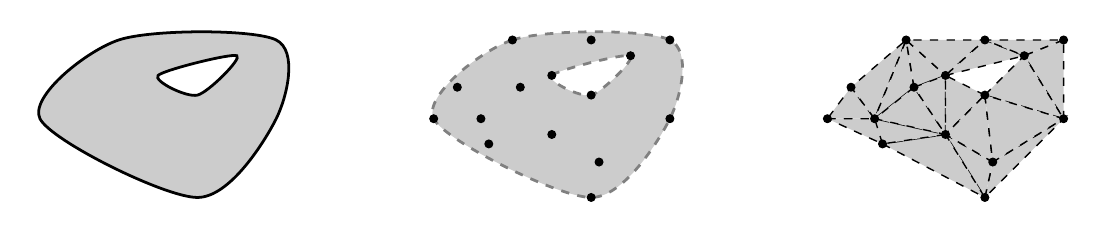
\begin{tikzpicture}
          \draw [black, line width=1, fill=black!20!white] plot [smooth cycle] coordinates {(0,0) (1,1) (3,1) (3,0) (2,-1)};
          \draw [black, line width=1, fill=white] plot [smooth cycle] coordinates {(2.5, 0.8)  (1.5, 0.55) (2, 0.3)     };
      %
      \draw [black!50!white, dashed, line width=1, fill=black!20!white] plot [smooth cycle] coordinates {(5,0) (6,1) (8,1) (8,0) (7,-1)};
          \draw [black!50!white, dashed, line width=1, fill=white] plot [smooth cycle] coordinates {(7, 0.3) (6.5, 0.55) (7.5, 0.8)};
      %
      \draw [black, line width=0.5, fill=black!20!white, circle, dashed  ] (10,0) -- (10.6, 0) -- (10.3, 0.4) -- cycle;
      \draw [black, line width=0.5, fill=black!20!white, circle, dashed  ] (10,0) -- (10.65, 0) -- (10.7, -0.32) -- cycle;
      \draw [black, line width=0.5, fill=black!20!white, circle, dashed  ] (10.6,0) -- (10.3, 0.4) -- (11, 1) -- cycle;
      \draw [black, line width=0.5, fill=black!20!white, circle, dashed  ] (10.6,0) -- (11.1, 0.4) -- (11, 1) -- cycle;
      \draw [black, line width=0.5, fill=black!20!white, circle, dashed  ] (11.5,0.55) -- (11.1, 0.4) -- (11, 1) -- cycle;
      \draw [black, line width=0.5, fill=black!20!white, circle, dashed  ] (11.5,0.55) -- (12, 1) -- (11, 1) -- cycle;
      \draw [black, line width=0.5, fill=black!20!white, circle, dashed  ] (11.5,0.55) -- (12.5, 0.8) -- (12, 1) -- cycle;
      \draw [black, line width=0.5, fill=black!20!white, circle, dashed  ] (13,1) -- (12.5, 0.8) -- (12, 1) -- cycle;
      \draw [black, line width=0.5, fill=black!20!white, circle, dashed  ] (13,1) -- (12.5, 0.8) -- (13, 0) -- cycle;
      \draw [black, line width=0.5, fill=black!20!white, circle, dashed  ] (12,0.3) -- (12.5, 0.8) -- (13, 0) -- cycle;
      \draw [black, line width=0.5, fill=black!20!white, circle, dashed  ] (12,-1) -- (12.1, -0.55) -- (13, 0) -- cycle;
      \draw [black, line width=0.5, fill=black!20!white, circle, dashed  ] (12,-1) -- (12.1, -0.55) -- (11.5, -0.2) -- cycle;
      \draw [black, line width=0.5, fill=black!20!white, circle, dashed  ] (10.7,-0.32) -- (12, -1) -- (11.5, -0.2) -- cycle;
      \draw [black, line width=0.5, fill=black!20!white, circle, dashed  ] (10.7,-0.32) -- (10.6, 0) -- (11.5, -0.2) -- cycle;
      \draw [black, line width=0.5, fill=black!20!white, circle, dashed  ] (11.1, 0.4) -- (10.6, 0) -- (11.5, -0.2) -- cycle;
      \draw [black, line width=0.5, fill=black!20!white, circle, dashed  ] (11.1, 0.4) -- (11.5, 0.55) -- (11.5, -0.2) -- cycle;
      \draw [black, line width=0.5, fill=black!20!white, circle, dashed  ] (12, 0.3) -- (11.5, 0.55) -- (11.5, -0.2) -- cycle;
      \draw [black, line width=0.5, fill=black!20!white, circle, dashed  ] (12, 0.3) -- (12.1, -0.55) -- (11.5, -0.2) -- cycle;
      \draw [black, line width=0.5, fill=black!20!white, circle, dashed  ] (12, 0.3) -- (12.1, -0.55) -- (13, 0) -- cycle;
      %   
      \node [draw=black,fill=black, shape=circle, scale=0.3] at (10, 0) {};
      \node [draw=black,fill=black, shape=circle, scale=0.3] at (11.1, 0.4) {};
      \node [draw=black,fill=black, shape=circle, scale=0.3] at (11.5, 0.55) {};
      \node [draw=black,fill=black, shape=circle, scale=0.3] at (11.5, -0.2) {};
      \node [draw=black,fill=black, shape=circle, scale=0.3] at (12, 0.3) {};
      \node [draw=black,fill=black, shape=circle, scale=0.3] at (12.1, -0.55) {};
      \node [draw=black,fill=black, shape=circle, scale=0.3] at (13, 0) {};
      \node [draw=black,fill=black, shape=circle, scale=0.3] at (10.7, -0.32) {};
      \node [draw=black,fill=black, shape=circle, scale=0.3] at (10.6, 0) {};
      \node [draw=black,fill=black, shape=circle, scale=0.3] at (12, -1) {};
      \node [draw=black,fill=black, shape=circle, scale=0.3] at (12.5, 0.8) {};
      \node [draw=black,fill=black, shape=circle, scale=0.3] at (10.3, 0.4) {};
      \node [draw=black,fill=black, shape=circle, scale=0.3] at (11, 1) {};
      \node [draw=black,fill=black, shape=circle, scale=0.3] at (12, 1) {};
      \node [draw=black,fill=black, shape=circle, scale=0.3] at (13, 1) {};
      %  
      \node [draw=black,fill=black, shape=circle, scale=0.3] at (5, 0) {};
      \node [draw=black,fill=black, shape=circle, scale=0.3] at (6.1, 0.4) {};
      \node [draw=black,fill=black, shape=circle, scale=0.3] at (6.5, 0.55) {};
      \node [draw=black,fill=black, shape=circle, scale=0.3] at (6.5, -0.2) {};
      \node [draw=black,fill=black, shape=circle, scale=0.3] at (7, 0.3) {};
      \node [draw=black,fill=black, shape=circle, scale=0.3] at (7.1, -0.55) {};
      \node [draw=black,fill=black, shape=circle, scale=0.3] at (8, 0) {};
      \node [draw=black,fill=black, shape=circle, scale=0.3] at (5.7, -0.32) {};
      \node [draw=black,fill=black, shape=circle, scale=0.3] at (5.6, 0) {};
      \node [draw=black,fill=black, shape=circle, scale=0.3] at (7, -1) {};
      \node [draw=black,fill=black, shape=circle, scale=0.3] at (7.5, 0.8) {};
      \node [draw=black,fill=black, shape=circle, scale=0.3] at (5.3, 0.4) {};
      \node [draw=black,fill=black, shape=circle, scale=0.3] at (6, 1) {};
      \node [draw=black,fill=black, shape=circle, scale=0.3] at (7, 1) {};
      \node [draw=black,fill=black, shape=circle, scale=0.3] at (8, 1) {};
      %
      
        \end{tikzpicture}
        }
      }
      \caption{Continuous and analogous discrete manifolds with one $1$-dimensional hole ($\dim \bar{\mc H}_1=1$). Left pane: the continuous manifold; center pane: the discretization with mesh vertices; right pane: a simplicial complex built upon the mesh. Triangles in the simplicial complex $\mc K$ are colored gray (right). 
      \label{fig:example_holes}
      }
    \end{figure}
    

Indeed, simplicial complex \( \mc K \) is not a manifold, although it may be seen as a discretization of the manifold, \Cref{fig:example_holes}. Moreover, one can show the convergence of the discrete homology group \( \mc H_k \) to its continuous counterpart in case of \( k = 1 \) in thermodynamic limit, \todo{refs}.



\subsubsection{ Elements of the Hodge decomposition as harmonic/vorticity/potential flow}
      \todo{ Maybe we will need here a quick discussion with connection to the continuous case }

Similarly, simplicial complex-specific case of the Hodge's decomposition, \Cref{thm:hodge_decomposition}, holds:
\begin{equation}
      \ds R^{m_k} = \lefteqn{\overbrace{\phantom{\im B_k^\top \oplus  \ker \left( B_k^\top B_k + B_{k+1} B_{k+1}^\top \right)}}^{\ker B_{k+1}^\top}} \im B_k^\top \oplus
      \underbrace{\ker \left( B_k^\top B_k + B_{k+1} B_{k+1}^\top \right) \oplus  \im B_{k+1}}_{\ker B_k}            
\end{equation}


\begin{definition}[Hodge Laplacian Operator]
      Let \( \mc K \) be a simplicial complex with corresponding boundary maps \( B_k \). Then due to \Cref{thm:two_kernels} and \Cref{lemma:hodge_kernels},
      \begin{equation}
            \mc H_k \cong \ker \left( B_k^\top B_k + B_{k+1} B_{k+1}^\top \right)
      \end{equation}
      Operator \( L_k =  B_k^\top B_k + B_{k+1} B_{k+1}^\top \) is known as \(k\)-th \emph{Hodge Laplacian} (or \emph{higher-order Laplacian}) operator. Two terms \( \Ld k =B_k^\top B_k  \) and \( \Lu k = B_{k+1} B_{k+1}^\top \) are known as \(k\)-th \emph{down}- and \emph{up}-Laplacians respectively.
\end{definition}

As established above, the homology group \( \mc H_k \cong \ker L_k \) consists of \emph{harmonic representative} or \emph{harmonic chains} (which name is explained by the fact of falling into the kernel of the corresponding Laplacian operator \( L_k \)). ELements of the remaining components of the decomposition can be described through the analogy with differential operator on simplicial complexes. For instance, 
\begin{enumerate}
      \item the conjugate boundary map \( B_1^\top \) is a discrete derivative on the graph: \( B_1^\top  [u_1, u_2 ] = [ u_2 ] - [u_1]\), hence \( B_1^\top  = \grad \) and \( B_1 =  -\diver \);
      \item the conjugate boundary map \( B_2^\top \) is a discrete \( \curl \) operator: \( B_2^\top [u_1, u_2, u_3 ] = [u_1, u_2] - [u_1, u_3]+[u_2, u_3] = [u_1, u_2] +[u_2, u_3] + [u_3, u_1]\); note that the fundamental lemma of homology de facto restates a widely known fact \( \curl \grad = 0 \);
      \item \(1\)-st order Hodge Laplacian operator then can be rewritten as a composition of the differential operators:
      \begin{equation}
            L_1 = - \grad \diver + \curl^* \curl = \Delta_1
      \end{equation}
      Operator \( \Delta_1 \) is known as a \emph{Helmholzian operator on graphs}, an analogue of the vector Laplacian, \cite{hanlonLaplacianMethod2002}.
\end{enumerate}

Following this, the elements of \( \im B_1^\top = \im ( \grad )\) are refered as \emph{potential flows} (since each element \( y_i\) of a vector \( \b y = B_1^\top \b x \) is a difference of potentials between some pair nodes \( \alpha \) and \( \beta \) forming the \(i\)-th edge); similarly, elements of \( \im B_2 = \im( \curl^*)\) are \emph{vector potentials} or \emph{vorticities}, and \( \ker B_1 \) and \( \ker B_2^\top \) are divergence- and curl-free flows respectively (a more low level discussion of these two subspaces is provided further).

\begin{remark}
      Consideration above provides a solid intuition but lacks clearly formality: indeed, in order to properly define graph's gradient, divergence and curl operators, one would need to discuss alternating functions on a graph (co-chains) and corresponding coboundary operator and cohomology,~\cite{limHodgeLaplaciansGraphs2020}, and show a direct connection with dicrete differential forms on manifolds. We choose to abstain from the introduction of another quite abstract entity since it should not affect the clarity of the numerical analysis of the Laplacian operators conducted further.
\end{remark}







\subsubsection{ Laplacian operators \( L_k \) }

The \(k\)-th order Hodge Laplacian operator \( L_k = B_k^\top B_k + B_{k+1} B_{k+1}^\top \) naturally joins the boundary relational information about simplices of differents orders in \( \mc K \) and describes the topological structure of the complex.

In its matrix form, \( L_k \) is symmetric ( \( L_k^\top = L_k\) ) and semi-positive definite ( \( \b x^\top L_k \b x = \b x^\top  B_k^\top B_k \b x  + \b x^\top B_{k+1} B_{k+1}^\top \b x = \| B_k \b x \|^2 + \| B_{k+1}^\top \b x \|^2 \ge 0 \) ) operator. Moreover, individual entries of down- and up-Laplacians \( \Ld k \) and \( \Lu k \) describe oriented adjacency of simplices in \( \V k \). Namely, two simplices \( \sigma, \sigma' \in \V k \) are down-adjacent by a common face \( \tau \in \V {k-1}\) with a similar  (so the orientation  of a common face agrees or disagrees with the orientation of \( \sigma \) and \( \sigma' \) simultaneously) and dissimilar orientation (otherwise); analogously, one can define an upper-adjacent pair \( \sigma, \sigma' \in \V k\) belonging to the same \( \tau \in \V {k+1} \). Then
\begin{equation}
      [ \Ld k ]_{ij} = \begin{cases}
            k+1, \qquad \text{if } i = j \\
            \phantom{k+}1, \qquad \text{if } i \ne j  \text{ and } \sigma_i, \sigma_j \text{ are upper-adjacent with similar orienation} \\
            \phantom{k}-1, \qquad \text{if } i \ne j \text{ and } \sigma_i, \sigma_j \text{ are upper-adjacent with dissimilar orienation} \\
            \phantom{k+}0 \qquad \text{otherwise}
      \end{cases}
\end{equation}
\begin{equation}
      [ \Lu k ]_{ij} = \begin{cases}
            \deg(\sigma_i), \qquad \text{if } i = j \\
            \phantom{k+}1, \qquad \text{if } i \ne j  \text{ and } \sigma_i, \sigma_j \text{ are down-adjacent with similar orienation} \\
            \phantom{k}-1, \qquad \text{if } i \ne j \text{ and } \sigma_i, \sigma_j \text{ are down-adjacent with dissimilar orienation} \\
            \phantom{k+}0 \qquad \text{otherwise}
      \end{cases}
\end{equation}
where \( \deg(\sigma_i) \) is the number of simplices in \( \V {k+1}\) having \( \sigma_i\) as a face.

\todo{figure?}

\subsubsection{ Classical Laplacian and its kernel elements }

Letting \( B_0 = 0 \) (the absence of the boundary of a node is reasonable), the \(0\)-order Hodge Laplacian \( L_0 \) is simply:
\begin{equation}
      L_0 = B_1 B_1^\top
\end{equation}


\subsubsection{ Kernel elements of \( L_k \) }

\todo{Some relation to the continuous case}

\paragraph{ Spreading and balancing as a mechanism of the non-local circulation}
















\section{ Weigthed and Normalised Boundary Operators}

\todo{definition and motivation of the weighting scheme}






Note that, from the definition \( \bar B_k= W_{k-1}^{-1} B_k W_k \) and \eqref{eq:Bk_Bk+1_0}, we immediately have that  \( \bar B_k\bar B_{k+1}=0 \). Thus, the group \( \bar {\mc H}_k = \ker \bar B_k / \im \bar B_{k+1} \) is well defined for any choice of positive weights  \( w_k \) and is isomorphic to \( \ker \bar L_k \). While the homology group may depend on the weights,  we observe below that its dimension does not. Precisely, we have 
\begin{proposition}
 \label[proposition]{thm:wHomGroup}
     The dimension of the homology groups of \( \mc K \) is not affected by the weights of its \( k \)-simplicies. Precisely, if \( W_k \) are positive diagonal matrices, we have
     \begin{equation}
         \dim \ker \bar B_k = \dim \ker B_k, \quad \dim \ker \bar B_k^\top = \dim \ker B_k^\top, \quad \dim \bar{\mc H}_k = \dim \mc H_k\, .
     \end{equation}
     Moreover, \( \ker B_k = W_k \ker \bar B_k \) and \( \ker B_k^\top = W_{k-1}^{-1} \ker \bar B_k^\top \).
\end{proposition}

\begin{proof}
Since \( W_k \) is an invertible diagonal matrix, 
\begin{equation*}
    \bar B_k \b x = 0 \iff W_{k-1}^{-1}B_k W_k \vec x =0 \iff B_k W_k \vec x =0. 
\end{equation*}
Hence, if \( \vec x \in \ker \bar B_k \), then \( W_k \vec x \in \ker B_k \), and, since \( W_k \) is bijective, \( \dim \ker \bar B_k = \dim \ker B_k \). Similarly, one observes that \( \dim \ker \bar B_k^\top = \dim \ker B_k^\top \).

Moreover, since \( \bar B_k \bar B_{k+1} =0 \), then \( \im \bar B_{k+1} \subseteq \ker \bar B_k \) and \( \im \bar B_k^\top \subseteq \ker \bar B_{k+1}^\top \). This yields \( \ker \bar B_k \cup \ker \bar B_{k+1}^\top = \mathbb{R}^{\mc V_k} = \ker B_k \cup \ker  B_{k+1}^\top\). Thus, for the homology group it holds:
\begin{equation*}
      \begin{aligned}
    \dim \bar {\mc H}_k & = \dim \left( \ker \bar B_k \cap \ker \bar B_{k+1}^\top \right)= \\
    & = \dim \ker \bar B_k + \dim \ker \bar B_{k+1}^\top - \dim \left( \ker \bar B_k \cup \ker \bar B_{k+1}^\top \right) = \\
    & = \dim \ker B_k + \dim \ker  B_{k+1}^\top - \dim \left( \ker  B_k \cup \ker  B_{k+1}^\top \right) = \dim \mc H_k
      \end{aligned}
\end{equation*}
\end{proof}


\todo{normalisation theorem}


